% ---------------------------------------------------------------------------
% Machine Learning Assignment 3 -- CVPR-format report.
% Uses the official CVPR author kit if cvpr.sty is in this folder (download it from
% the CVPR author-kit GitHub repository and copy cvpr.sty + ieeenat_fullname.bst here).
% Otherwise falls back to an equivalent two-column 10pt layout so it always compiles.
% All numbers come from generated/numbers.tex and generated/*.tex (see src/make_report_assets.py).
% ---------------------------------------------------------------------------
\documentclass[10pt,twocolumn,letterpaper]{article}
\IfFileExists{cvpr.sty}{\usepackage[pagenumbers]{cvpr}}{%
  \usepackage[letterpaper,top=1in,bottom=1in,left=0.75in,right=0.75in,columnsep=0.3125in]{geometry}%
  \usepackage{times}}
\usepackage{graphicx,booktabs,amsmath,amssymb,xcolor,url,adjustbox}
\usepackage[hidelinks]{hyperref}
\usepackage[capitalize]{cleveref}

% ---- generated numbers (smoke build: pdflatex "\def\smoke{1}% ---------------------------------------------------------------------------
% Machine Learning Assignment 3 -- CVPR-format report.
% Uses the official CVPR author kit if cvpr.sty is in this folder (download it from
% the CVPR author-kit GitHub repository and copy cvpr.sty + ieeenat_fullname.bst here).
% Otherwise falls back to an equivalent two-column 10pt layout so it always compiles.
% All numbers come from generated/numbers.tex and generated/*.tex (see src/make_report_assets.py).
% ---------------------------------------------------------------------------
\documentclass[10pt,twocolumn,letterpaper]{article}
\IfFileExists{cvpr.sty}{\usepackage[pagenumbers]{cvpr}}{%
  \usepackage[letterpaper,top=1in,bottom=1in,left=0.75in,right=0.75in,columnsep=0.3125in]{geometry}%
  \usepackage{times}}
\usepackage{graphicx,booktabs,amsmath,amssymb,xcolor,url,adjustbox}
\usepackage[hidelinks]{hyperref}
\usepackage[capitalize]{cleveref}

% ---- generated numbers (smoke build: pdflatex "\def\smoke{1}% ---------------------------------------------------------------------------
% Machine Learning Assignment 3 -- CVPR-format report.
% Uses the official CVPR author kit if cvpr.sty is in this folder (download it from
% the CVPR author-kit GitHub repository and copy cvpr.sty + ieeenat_fullname.bst here).
% Otherwise falls back to an equivalent two-column 10pt layout so it always compiles.
% All numbers come from generated/numbers.tex and generated/*.tex (see src/make_report_assets.py).
% ---------------------------------------------------------------------------
\documentclass[10pt,twocolumn,letterpaper]{article}
\IfFileExists{cvpr.sty}{\usepackage[pagenumbers]{cvpr}}{%
  \usepackage[letterpaper,top=1in,bottom=1in,left=0.75in,right=0.75in,columnsep=0.3125in]{geometry}%
  \usepackage{times}}
\usepackage{graphicx,booktabs,amsmath,amssymb,xcolor,url,adjustbox}
\usepackage[hidelinks]{hyperref}
\usepackage[capitalize]{cleveref}

% ---- generated numbers (smoke build: pdflatex "\def\smoke{1}% ---------------------------------------------------------------------------
% Machine Learning Assignment 3 -- CVPR-format report.
% Uses the official CVPR author kit if cvpr.sty is in this folder (download it from
% the CVPR author-kit GitHub repository and copy cvpr.sty + ieeenat_fullname.bst here).
% Otherwise falls back to an equivalent two-column 10pt layout so it always compiles.
% All numbers come from generated/numbers.tex and generated/*.tex (see src/make_report_assets.py).
% ---------------------------------------------------------------------------
\documentclass[10pt,twocolumn,letterpaper]{article}
\IfFileExists{cvpr.sty}{\usepackage[pagenumbers]{cvpr}}{%
  \usepackage[letterpaper,top=1in,bottom=1in,left=0.75in,right=0.75in,columnsep=0.3125in]{geometry}%
  \usepackage{times}}
\usepackage{graphicx,booktabs,amsmath,amssymb,xcolor,url,adjustbox}
\usepackage[hidelinks]{hyperref}
\usepackage[capitalize]{cleveref}

% ---- generated numbers (smoke build: pdflatex "\def\smoke{1}\input{main}") ----
\ifdefined\smoke
  \def\gen{generated_smoke}\graphicspath{{../figures_smoke/}}
\else
  \def\gen{generated}\graphicspath{{../figures/}}
\fi
\input{\gen/numbers.tex}
\providecommand{\QtwoBlockC}{--}

% ---- conclusions are generated by the pre-registered decision rules in src/conclusions.py ----
\input{\gen/conclusions.tex}
\newcommand{\pred}[1]{\textit{Prediction (fixed before training, PREDICTIONS.md):} #1}

\title{Inductive Bias, Memorisation, Representations and Margins on CIFAR10}
\author{\StudentName\\ Roll no.\ \RollNumber\\ {\small Code: \RepoURL\quad Commit: \texttt{\CommitHash}}}
\date{}

\begin{document}
\maketitle

\begin{abstract}
We study why multilayer perceptrons (MLPs) underperform on CIFAR10 and test the explanation with equal-budget
controls, a pixel-permutation ablation and a label-noise memorisation experiment tracked across training.
We then compare a parameter-matched CNN with the MLP, probe what the CNN relies on with per-image block shuffles,
study convolutional autoencoders (bottleneck size, denoising, linear probes), and analyse SVMs and clustering on a
fixed learned representation. Every reported number is generated from the logged runs in the repository.
\end{abstract}

% =========================================================================== 1
\section{Common setup}
\textbf{Data.} The 50{,}000 CIFAR10 training images are split once into a stratified 45{,}000/5{,}000 train/validation
split with \texttt{sklearn.train\_test\_split(stratify=y)} and seed \SplitSeed{} (all digits of roll number \RollNumber,
in order). The split indices are saved in \texttt{splits/cifar10\_split.npz} and reused by every experiment.
Per-channel mean/std are computed on the 45k training images only. The validation set is the only signal for any choice
(learning rate, checkpoint epoch, bottleneck, kernel, $C$, clustering method, $k$). The official test set is evaluated
only after a choice is fixed.

\textbf{Shared training protocol.} Every classifier (all MLPs, the Patch-MLP and all CNNs) is trained by the same function
(\texttt{src/common.py:train\_classifier}): AdamW, weight decay $5\cdot10^{-4}$, batch 256, one warm-up epoch then cosine
decay, no data augmentation, and the checkpoint with the best validation accuracy. No augmentation is a deliberate choice:
random crops/flips inject a translation prior into the \emph{data}, which would confound the inductive-bias questions in
Q1/Q2. Every model receives the same tuning budget: the LR grid $\{10^{-3},3\cdot10^{-4}\}$ is searched at seed 0, and
the selected LR is re-run with seeds 1 and 2; we report mean$\pm$sd over three seeds.

\textbf{Reuse.} Models are cached by name in \texttt{results/checkpoints}. Reused components are marked where used:
the Q1(a) MLP and its pixel-permuted runs are reused in Q2; the Q2(a) seed-0 CNN is the fixed classifier in Q3(b);
the Q3 encoders provide the Q4 representation.

% =========================================================================== 2
\section{Q1: Why MLPs struggle, and memorisation}
\subsection{(a) Separating the explanations}
\textbf{Chosen reason (H\textsubscript{bias}).} A fully connected layer treats the 3072 inputs as an unordered vector.
It has no locality and no weight sharing, so a detector learned at one image position cannot be reused at another, and
neighbouring pixels are not known to be related. With 45k images the MLP can fit the training set but generalises poorly.

\textbf{Competing explanations.} H\textsubscript{cap}: the MLP lacks capacity and \emph{underfits}.
H\textsubscript{opt}: the one-hidden-layer shape is the problem and a deeper MLP of the same size would fix it.

\textbf{Design.} Three models are matched to the same parameter budget by binary-searching their width
(\cref{tab:q1spec}). The plain MLP is the baseline. The deep MLP keeps the budget and only changes depth (tests
H\textsubscript{opt}). The Patch-MLP is still built only from Linear layers. Its single change is a minimal spatial
prior: one small MLP, shared across positions, embeds every $4\times4$ patch, and a fully connected head then reads all
patch embeddings (tests H\textsubscript{bias}). Two further diagnostics are used. (i) A width sweep of the plain MLP: if
H\textsubscript{cap} held, validation accuracy would keep rising with width. Here the parameter count varies by design,
and only validation is used. (ii) A fixed pixel permutation applied to train, validation and test. If the Patch-MLP's gain
comes from spatial structure, it must vanish under permutation, while the plain MLP's accuracy is unchanged.

\textbf{Fairness.} We call the comparison fair when parameters are within 2\%, the data and preprocessing are identical,
and the epochs, optimiser, schedule, LR grid, seeds and selection rule are identical. Compute (MACs) is not matched: weight
sharing reuses parameters, and that reuse is the property under test.

\input{\gen/q1a_spec.tex}
\input{\gen/q1a.tex}
\input{\gen/q1a_capacity.tex}
\begin{figure*}[t]\centering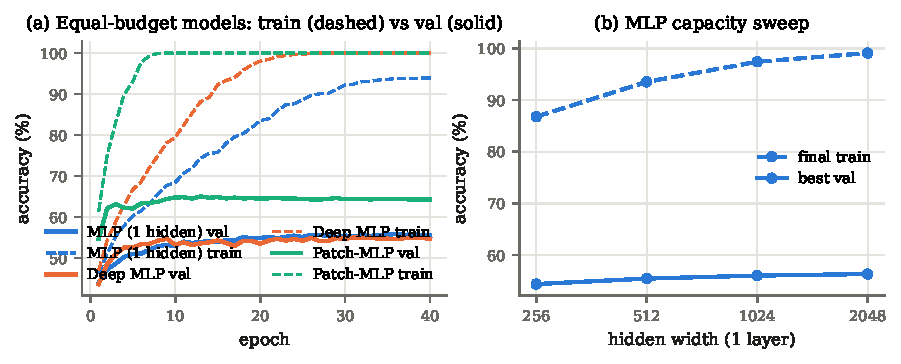
\includegraphics[width=\textwidth]{q1a_curves.pdf}
\caption{Q1(a) seed-0 training curves at the selected LR (left) and the MLP width sweep (right).}\label{fig:q1a}\end{figure*}

\textbf{Evidence.} The plain MLP reaches \QoneTrainmlp\% training accuracy at its selected epoch but only \QoneValmlp\%
validation accuracy. Its test accuracy is \QoneTestmlp\%. Deep MLP: \QoneTestmlpdeep\%; Patch-MLP: \QoneTestpatchmlp\%
(\cref{tab:q1a,tab:q1cap,fig:q1a}). Each hypothesis is judged by the rule fixed in \texttt{PREDICTIONS.md}.
\ConcQoneA

\subsection{(b) Is structure learned before memorisation?}
\textbf{Setting.} A \QoneBParams-parameter MLP (two hidden layers of width 2048) has more than enough capacity to fit 45k
examples. It is trained for 150 epochs at a constant LR with no weight decay. A fixed 40\% of the training labels (seeded)
are replaced by a uniformly random \emph{wrong} class; these examples cannot generalise by construction. At every epoch we
measure, on the training set: accuracy on the clean subset; agreement of the noisy subset with its noisy label
(memorisation); agreement of the noisy subset with its hidden true label (structure); and clean validation accuracy. A
clean-label run with an identical protocol is the control. We also record, for every example, the epoch from which it
stays fitted until the end of training (\cref{fig:q1b}b).

\input{\gen/q1b.tex}
\begin{figure*}[t]\centering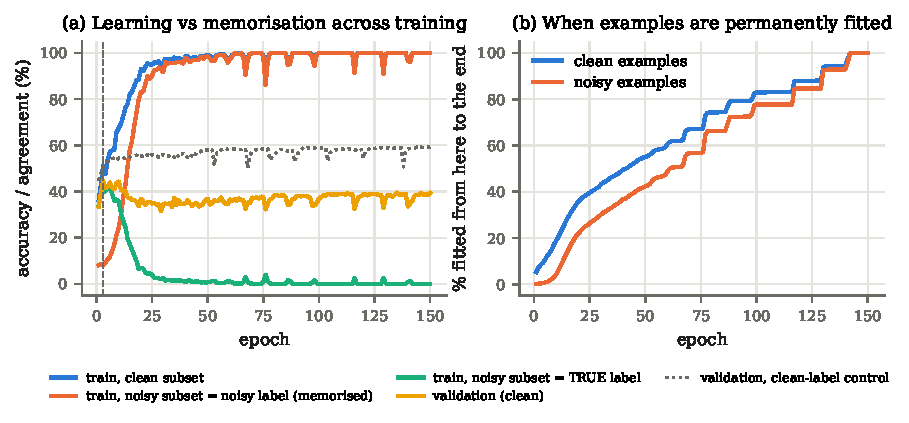
\includegraphics[width=\textwidth]{q1b_memorisation.pdf}
\caption{Q1(b) per-epoch measurements under 40\% label noise. The dashed vertical line marks peak validation accuracy.}\label{fig:q1b}\end{figure*}

\textbf{Evidence.} Validation accuracy peaks at epoch \QoneBPeakEpoch{} (\QoneBPeakVal\%). At that epoch only
\QoneBPeakNoisyFit\% of the corrupted examples are predicted as their noisy label, while \QoneBPeakNoisyTrue\% are
predicted as their \emph{true} class. The noisy-fit fraction first exceeds 50\% at epoch \QoneBOnsetFifty. \ConcQoneB{} \Cref{fig:q1b}b shows the same
ordering per example: the epoch from which an example stays fitted is early for clean examples and late for corrupted
ones. The test accuracy of the val-selected checkpoint
is \QoneBTest\%.

% =========================================================================== 3
\section{Q2: CNN vs MLP}
\textbf{Fairness criterion (fixed before training).} The CNN's width is binary-searched so that its parameter count
matches the Q1 MLP (\QtwoCNNparams{} vs \QtwoMLPparams). Everything else follows the shared protocol of Q1. The Q1(a)
plain MLP and its runs are \emph{reused} unchanged as the Q2 MLP. The CNN uses about \QtwoMACratio$\times$ more MACs per
image; we report this rather than hide it.

\input{\gen/q2.tex}

\textbf{(a) Result and proposed reason.} The CNN reaches \QtwoCNNclean\% test accuracy and the MLP \QtwoMLPclean\%.
The proposed reason is the same spatial prior identified in Q1: local receptive fields with shared weights reuse one
feature detector at every position, so far fewer examples are needed per feature.

\textbf{(b) Spatial disturbance.} We apply one fixed permutation of the 1024 pixel positions, identical for every
training, validation and test image. RGB triplets move together, so all pixel values and colours are preserved exactly.
\pred{the MLP is unchanged within seed noise, because a fixed input permutation can be absorbed into its first layer; the
CNN falls to roughly the MLP level or below.} Observed: MLP \QtwoMLPperm\%, CNN \QtwoCNNperm\%. \ConcQtwoB

\textbf{(c) Which spatial information does the CNN use?}
E\textsubscript{local}: the CNN classifies from local texture and colour statistics, like a bag of local features.
E\textsubscript{global}: it needs the global arrangement of object parts. We cut every image into $b\times b$ tiles
($b\in\{16,8,4\}$) and shuffle the tiles with a permutation that differs per image (deterministic from a seed). This keeps
the content inside each tile and destroys the global layout. The CNN is retrained per condition. The identical
transformation (same operator, block size and seeded generator) is applied to training, validation and test images; as with
any random transformation, only the per-image draw differs. \pred{under E\textsubscript{local}, accuracy and confidence largely
survive at $b=16$ and $b=8$ and fall at $b=4$, when tiles become smaller than parts. Under E\textsubscript{global}, there is
already a large drop at $b=16$.}

\input{\gen/q2_conf.tex}
\begin{figure*}[t]\centering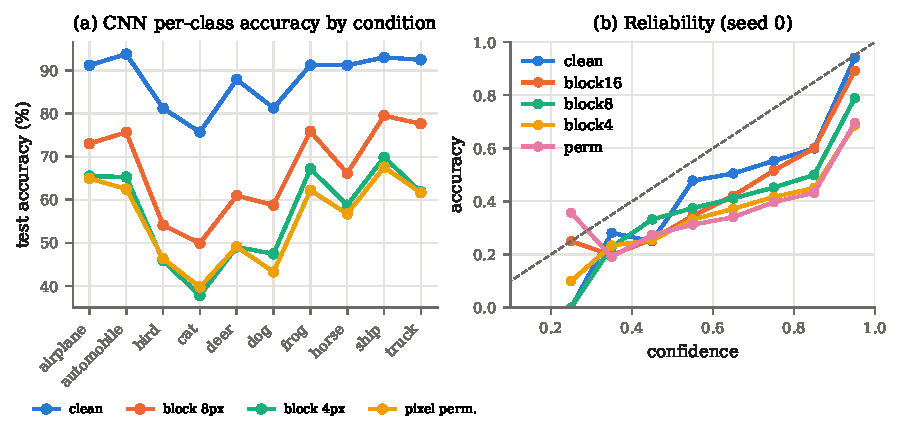
\includegraphics[width=\textwidth]{q2_analysis.pdf}
\caption{Q2(c): per-class test accuracy and reliability diagrams for the CNN across conditions.}\label{fig:q2}\end{figure*}

Decision rule (pre-registered): E\textsubscript{local} if the drop at 16\,px is $<$40\% of the drop at 4\,px,
E\textsubscript{global} if $\ge$60\%, otherwise both. \ConcQtwoC

\textbf{Conclusion linking the three experiments.} \ConcQtwoLink

% =========================================================================== 4
\section{Q3: Autoencoders}
\textbf{(a) Bottleneck capacity.} The three ConvAEs share one encoder (three stride-2 conv layers, $32\to4$ px, 2048
values), a Linear bottleneck of size $d\in\{16,128,1024\}$ and a mirrored decoder with a sigmoid output. Only $d$ changes.
Training uses MSE on $[0,1]$ pixels, AdamW at LR $10^{-3}$, cosine decay and 40 epochs; the checkpoint is the epoch with
the lowest validation MSE. Selection rule: lowest validation MSE. The selected model is $d=\QthreeSel$, with test MSE
\QthreeTestMSE{} (PSNR \QthreeTestPSNR{} dB).
\input{\gen/q3a.tex}

\textbf{(b) Denoising.} Corruption: additive Gaussian noise, $\sigma=0.2$, clipped to $[0,1]$. Reconstruction can
plausibly help because the noise is independent per pixel while natural images are spatially smooth. Protocol: the DAE has
the same architecture as the selected AE. Its input is a freshly noised training image in every batch, the target is the
clean image, and no labels are used. Validation and test noise are drawn once with fixed seeds. The fixed classifier is the
Q2(a) seed-0 CNN (\emph{reused}, never fine-tuned).
\input{\gen/q3b.tex}
Decision rule (pre-registered): the DAE ``recovers the information the classifier needs'' if it closes $\ge$50\% of
the clean--noisy gap \emph{and} comes within 3\,pp of the ``clean AE on clean'' ceiling. \ConcQthreeB

\textbf{(c) Class information vs reconstruction.} The encoders are frozen. Bottleneck features of the three AEs, the DAE
and a randomly initialised encoder (control) are classified with an L2-regularised linear softmax probe (strength chosen
on validation) and with 20-NN.
\input{\gen/q3c.tex}
\begin{figure*}[t]\centering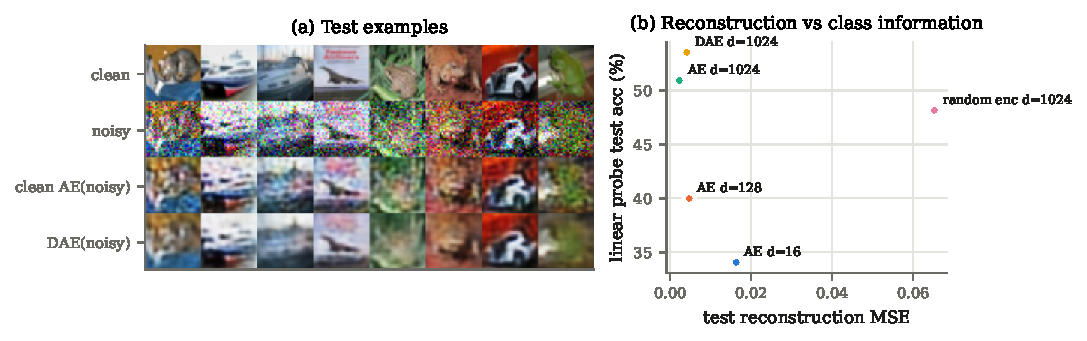
\includegraphics[width=0.85\textwidth]{q3.pdf}
\caption{Q3: test reconstructions (left), and linear-probe accuracy against reconstruction error (right).}\label{fig:q3}\end{figure*}
Decision rule: the two quantities ``agree'' if ranking the three AEs by test MSE gives the same order as ranking them
by probe accuracy, and the DAE does not reverse the relation. \ConcQthreeC

% =========================================================================== 5
\section{Q4 (bonus): SVMs and clustering}
\textbf{Representation.} Chosen before any SVM is fitted: the Q3 encoder with the highest linear-probe \emph{validation}
accuracy, \emph{\QfourRep}. Features are standardised with statistics from the subset. Because of cost, a fixed stratified
subset of \QfourSubset{} training images is drawn with the split seed before model selection and saved
(\texttt{splits/q4\_subset.npz}). It is used for every SVM; validation uses all 5k images.

\textbf{(a) $C$ and kernel.} Linear, cubic-polynomial and RBF kernels ($\gamma=$\texttt{scale}), with
$C\in\{10^{-2},\dots,10^{3}\}$ (five orders of magnitude).
\input{\gen/q4a.tex}
\begin{figure*}[t]\centering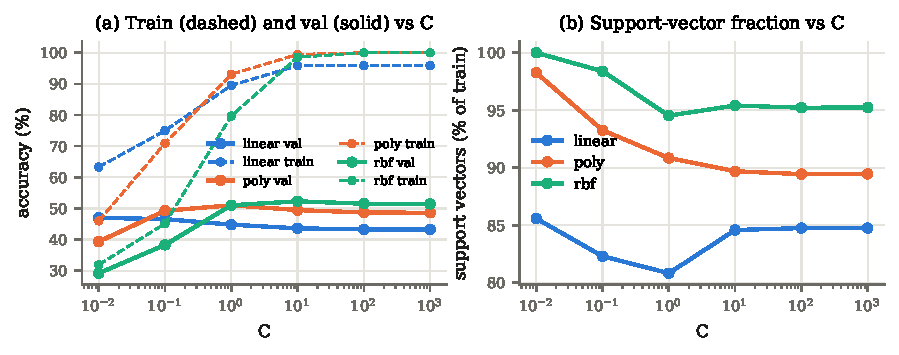
\includegraphics[width=\textwidth]{q4a.pdf}
\caption{Q4(a) validation/training accuracy and support-vector fraction against $C$ for each kernel.}\label{fig:q4a}\end{figure*}
\ConcQfourA

\textbf{(b) Difficult pairs.} The three most-confused test pairs are analysed with the pair's own one-vs-one decision
function $f_{ij}$, extracted from the fitted SVC and verified numerically against \texttt{decision\_function}.
\input{\gen/q4b.tex}
\begin{figure}[t]\centering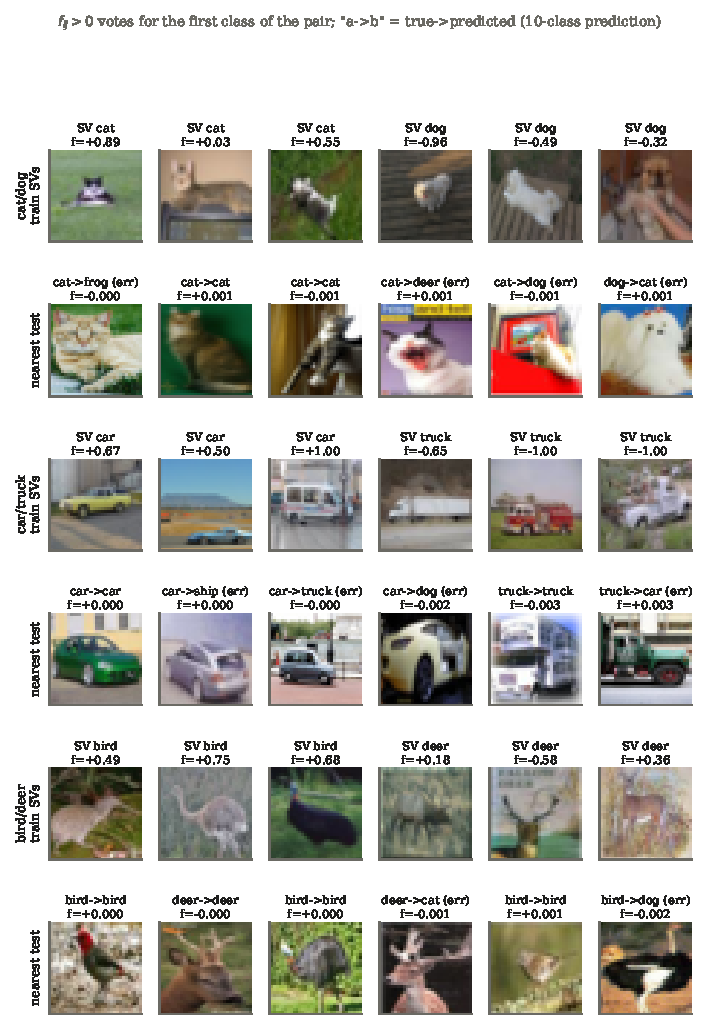
\includegraphics[width=\linewidth]{q4b_pairs.pdf}
\caption{Q4(b) training support vectors with the largest $|\alpha|$ and the test images closest to the $i$/$j$ boundary.}\label{fig:q4b}\end{figure}
\ConcQfourB

\textbf{(c) Clustering.} K-means and diagonal-covariance GMMs are fitted on training representations without labels, for
$k\in\{5,8,10,12,15,20\}$. The method and $k$ are chosen by the highest validation silhouette (label-free). The selected
model (\QfourClu) assigns the test representations; labels are used only afterwards. Test ARI is \QfourARI, NMI \QfourNMI,
purity \QfourPurity\%, and accuracy after a train-label majority mapping \QfourMapAcc\%.
\input{\gen/q4c_sel.tex}
\begin{figure}[t]\centering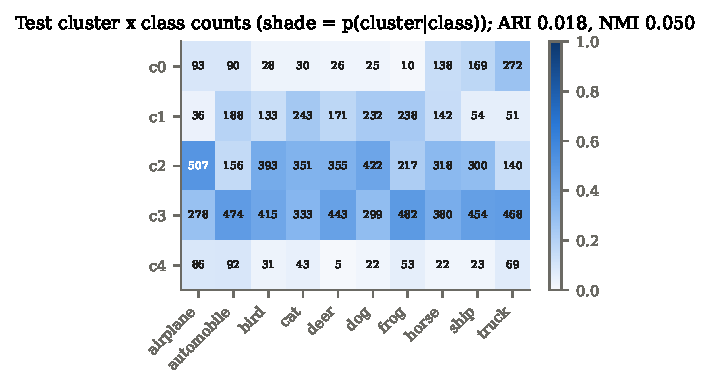
\includegraphics[width=\linewidth]{q4c_contingency.pdf}
\caption{Q4(c) test cluster-to-class contingency table.}\label{fig:q4c}\end{figure}
\input{\gen/q4c_perclass.tex}
\ConcQfourC

% =========================================================================== 6
\section{Reproducibility}
\texttt{bash scripts/run\_all.sh} reproduces every number. The environment is in \texttt{environment.yml}; split indices,
the Q4 subset, configs, per-epoch logs (\texttt{results/runs/*.json}) and figure scripts are in the repository at the
commit shown on page~1.

\end{document}
") ----
\ifdefined\smoke
  \def\gen{generated_smoke}\graphicspath{{../figures_smoke/}}
\else
  \def\gen{generated}\graphicspath{{../figures/}}
\fi
\input{\gen/numbers.tex}
\providecommand{\QtwoBlockC}{--}

% ---- conclusions are generated by the pre-registered decision rules in src/conclusions.py ----
\input{\gen/conclusions.tex}
\newcommand{\pred}[1]{\textit{Prediction (fixed before training, PREDICTIONS.md):} #1}

\title{Inductive Bias, Memorisation, Representations and Margins on CIFAR10}
\author{\StudentName\\ Roll no.\ \RollNumber\\ {\small Code: \RepoURL\quad Commit: \texttt{\CommitHash}}}
\date{}

\begin{document}
\maketitle

\begin{abstract}
We study why multilayer perceptrons (MLPs) underperform on CIFAR10 and test the explanation with equal-budget
controls, a pixel-permutation ablation and a label-noise memorisation experiment tracked across training.
We then compare a parameter-matched CNN with the MLP, probe what the CNN relies on with per-image block shuffles,
study convolutional autoencoders (bottleneck size, denoising, linear probes), and analyse SVMs and clustering on a
fixed learned representation. Every reported number is generated from the logged runs in the repository.
\end{abstract}

% =========================================================================== 1
\section{Common setup}
\textbf{Data.} The 50{,}000 CIFAR10 training images are split once into a stratified 45{,}000/5{,}000 train/validation
split with \texttt{sklearn.train\_test\_split(stratify=y)} and seed \SplitSeed{} (all digits of roll number \RollNumber,
in order). The split indices are saved in \texttt{splits/cifar10\_split.npz} and reused by every experiment.
Per-channel mean/std are computed on the 45k training images only. The validation set is the only signal for any choice
(learning rate, checkpoint epoch, bottleneck, kernel, $C$, clustering method, $k$). The official test set is evaluated
only after a choice is fixed.

\textbf{Shared training protocol.} Every classifier (all MLPs, the Patch-MLP and all CNNs) is trained by the same function
(\texttt{src/common.py:train\_classifier}): AdamW, weight decay $5\cdot10^{-4}$, batch 256, one warm-up epoch then cosine
decay, no data augmentation, and the checkpoint with the best validation accuracy. No augmentation is a deliberate choice:
random crops/flips inject a translation prior into the \emph{data}, which would confound the inductive-bias questions in
Q1/Q2. Every model receives the same tuning budget: the LR grid $\{10^{-3},3\cdot10^{-4}\}$ is searched at seed 0, and
the selected LR is re-run with seeds 1 and 2; we report mean$\pm$sd over three seeds.

\textbf{Reuse.} Models are cached by name in \texttt{results/checkpoints}. Reused components are marked where used:
the Q1(a) MLP and its pixel-permuted runs are reused in Q2; the Q2(a) seed-0 CNN is the fixed classifier in Q3(b);
the Q3 encoders provide the Q4 representation.

% =========================================================================== 2
\section{Q1: Why MLPs struggle, and memorisation}
\subsection{(a) Separating the explanations}
\textbf{Chosen reason (H\textsubscript{bias}).} A fully connected layer treats the 3072 inputs as an unordered vector.
It has no locality and no weight sharing, so a detector learned at one image position cannot be reused at another, and
neighbouring pixels are not known to be related. With 45k images the MLP can fit the training set but generalises poorly.

\textbf{Competing explanations.} H\textsubscript{cap}: the MLP lacks capacity and \emph{underfits}.
H\textsubscript{opt}: the one-hidden-layer shape is the problem and a deeper MLP of the same size would fix it.

\textbf{Design.} Three models are matched to the same parameter budget by binary-searching their width
(\cref{tab:q1spec}). The plain MLP is the baseline. The deep MLP keeps the budget and only changes depth (tests
H\textsubscript{opt}). The Patch-MLP is still built only from Linear layers. Its single change is a minimal spatial
prior: one small MLP, shared across positions, embeds every $4\times4$ patch, and a fully connected head then reads all
patch embeddings (tests H\textsubscript{bias}). Two further diagnostics are used. (i) A width sweep of the plain MLP: if
H\textsubscript{cap} held, validation accuracy would keep rising with width. Here the parameter count varies by design,
and only validation is used. (ii) A fixed pixel permutation applied to train, validation and test. If the Patch-MLP's gain
comes from spatial structure, it must vanish under permutation, while the plain MLP's accuracy is unchanged.

\textbf{Fairness.} We call the comparison fair when parameters are within 2\%, the data and preprocessing are identical,
and the epochs, optimiser, schedule, LR grid, seeds and selection rule are identical. Compute (MACs) is not matched: weight
sharing reuses parameters, and that reuse is the property under test.

\input{\gen/q1a_spec.tex}
\input{\gen/q1a.tex}
\input{\gen/q1a_capacity.tex}
\begin{figure*}[t]\centering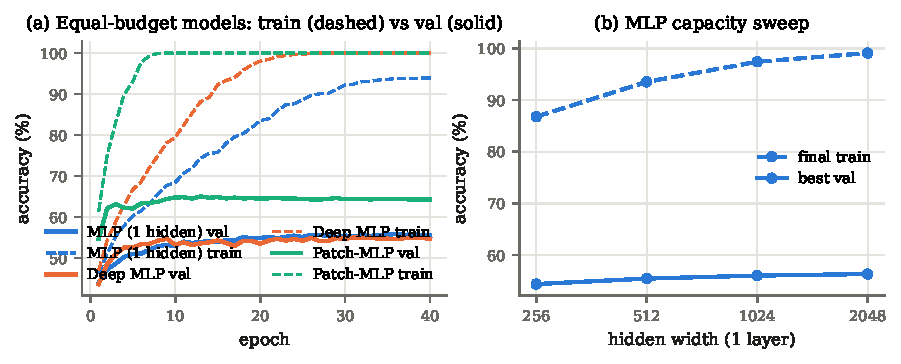
\includegraphics[width=\textwidth]{q1a_curves.pdf}
\caption{Q1(a) seed-0 training curves at the selected LR (left) and the MLP width sweep (right).}\label{fig:q1a}\end{figure*}

\textbf{Evidence.} The plain MLP reaches \QoneTrainmlp\% training accuracy at its selected epoch but only \QoneValmlp\%
validation accuracy. Its test accuracy is \QoneTestmlp\%. Deep MLP: \QoneTestmlpdeep\%; Patch-MLP: \QoneTestpatchmlp\%
(\cref{tab:q1a,tab:q1cap,fig:q1a}). Each hypothesis is judged by the rule fixed in \texttt{PREDICTIONS.md}.
\ConcQoneA

\subsection{(b) Is structure learned before memorisation?}
\textbf{Setting.} A \QoneBParams-parameter MLP (two hidden layers of width 2048) has more than enough capacity to fit 45k
examples. It is trained for 150 epochs at a constant LR with no weight decay. A fixed 40\% of the training labels (seeded)
are replaced by a uniformly random \emph{wrong} class; these examples cannot generalise by construction. At every epoch we
measure, on the training set: accuracy on the clean subset; agreement of the noisy subset with its noisy label
(memorisation); agreement of the noisy subset with its hidden true label (structure); and clean validation accuracy. A
clean-label run with an identical protocol is the control. We also record, for every example, the epoch from which it
stays fitted until the end of training (\cref{fig:q1b}b).

\input{\gen/q1b.tex}
\begin{figure*}[t]\centering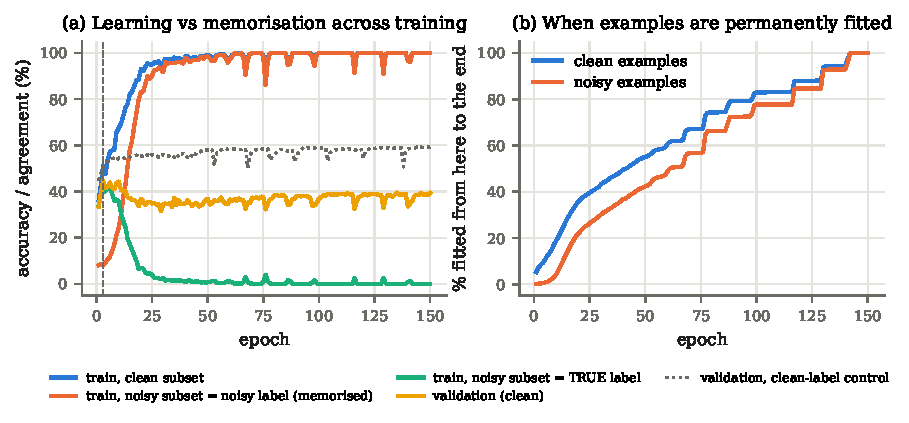
\includegraphics[width=\textwidth]{q1b_memorisation.pdf}
\caption{Q1(b) per-epoch measurements under 40\% label noise. The dashed vertical line marks peak validation accuracy.}\label{fig:q1b}\end{figure*}

\textbf{Evidence.} Validation accuracy peaks at epoch \QoneBPeakEpoch{} (\QoneBPeakVal\%). At that epoch only
\QoneBPeakNoisyFit\% of the corrupted examples are predicted as their noisy label, while \QoneBPeakNoisyTrue\% are
predicted as their \emph{true} class. The noisy-fit fraction first exceeds 50\% at epoch \QoneBOnsetFifty. \ConcQoneB{} \Cref{fig:q1b}b shows the same
ordering per example: the epoch from which an example stays fitted is early for clean examples and late for corrupted
ones. The test accuracy of the val-selected checkpoint
is \QoneBTest\%.

% =========================================================================== 3
\section{Q2: CNN vs MLP}
\textbf{Fairness criterion (fixed before training).} The CNN's width is binary-searched so that its parameter count
matches the Q1 MLP (\QtwoCNNparams{} vs \QtwoMLPparams). Everything else follows the shared protocol of Q1. The Q1(a)
plain MLP and its runs are \emph{reused} unchanged as the Q2 MLP. The CNN uses about \QtwoMACratio$\times$ more MACs per
image; we report this rather than hide it.

\input{\gen/q2.tex}

\textbf{(a) Result and proposed reason.} The CNN reaches \QtwoCNNclean\% test accuracy and the MLP \QtwoMLPclean\%.
The proposed reason is the same spatial prior identified in Q1: local receptive fields with shared weights reuse one
feature detector at every position, so far fewer examples are needed per feature.

\textbf{(b) Spatial disturbance.} We apply one fixed permutation of the 1024 pixel positions, identical for every
training, validation and test image. RGB triplets move together, so all pixel values and colours are preserved exactly.
\pred{the MLP is unchanged within seed noise, because a fixed input permutation can be absorbed into its first layer; the
CNN falls to roughly the MLP level or below.} Observed: MLP \QtwoMLPperm\%, CNN \QtwoCNNperm\%. \ConcQtwoB

\textbf{(c) Which spatial information does the CNN use?}
E\textsubscript{local}: the CNN classifies from local texture and colour statistics, like a bag of local features.
E\textsubscript{global}: it needs the global arrangement of object parts. We cut every image into $b\times b$ tiles
($b\in\{16,8,4\}$) and shuffle the tiles with a permutation that differs per image (deterministic from a seed). This keeps
the content inside each tile and destroys the global layout. The CNN is retrained per condition. The identical
transformation (same operator, block size and seeded generator) is applied to training, validation and test images; as with
any random transformation, only the per-image draw differs. \pred{under E\textsubscript{local}, accuracy and confidence largely
survive at $b=16$ and $b=8$ and fall at $b=4$, when tiles become smaller than parts. Under E\textsubscript{global}, there is
already a large drop at $b=16$.}

\input{\gen/q2_conf.tex}
\begin{figure*}[t]\centering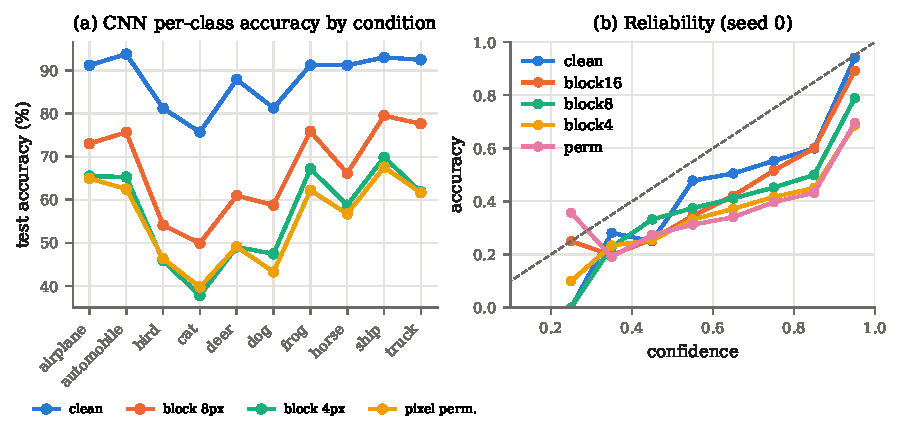
\includegraphics[width=\textwidth]{q2_analysis.pdf}
\caption{Q2(c): per-class test accuracy and reliability diagrams for the CNN across conditions.}\label{fig:q2}\end{figure*}

Decision rule (pre-registered): E\textsubscript{local} if the drop at 16\,px is $<$40\% of the drop at 4\,px,
E\textsubscript{global} if $\ge$60\%, otherwise both. \ConcQtwoC

\textbf{Conclusion linking the three experiments.} \ConcQtwoLink

% =========================================================================== 4
\section{Q3: Autoencoders}
\textbf{(a) Bottleneck capacity.} The three ConvAEs share one encoder (three stride-2 conv layers, $32\to4$ px, 2048
values), a Linear bottleneck of size $d\in\{16,128,1024\}$ and a mirrored decoder with a sigmoid output. Only $d$ changes.
Training uses MSE on $[0,1]$ pixels, AdamW at LR $10^{-3}$, cosine decay and 40 epochs; the checkpoint is the epoch with
the lowest validation MSE. Selection rule: lowest validation MSE. The selected model is $d=\QthreeSel$, with test MSE
\QthreeTestMSE{} (PSNR \QthreeTestPSNR{} dB).
\input{\gen/q3a.tex}

\textbf{(b) Denoising.} Corruption: additive Gaussian noise, $\sigma=0.2$, clipped to $[0,1]$. Reconstruction can
plausibly help because the noise is independent per pixel while natural images are spatially smooth. Protocol: the DAE has
the same architecture as the selected AE. Its input is a freshly noised training image in every batch, the target is the
clean image, and no labels are used. Validation and test noise are drawn once with fixed seeds. The fixed classifier is the
Q2(a) seed-0 CNN (\emph{reused}, never fine-tuned).
\input{\gen/q3b.tex}
Decision rule (pre-registered): the DAE ``recovers the information the classifier needs'' if it closes $\ge$50\% of
the clean--noisy gap \emph{and} comes within 3\,pp of the ``clean AE on clean'' ceiling. \ConcQthreeB

\textbf{(c) Class information vs reconstruction.} The encoders are frozen. Bottleneck features of the three AEs, the DAE
and a randomly initialised encoder (control) are classified with an L2-regularised linear softmax probe (strength chosen
on validation) and with 20-NN.
\input{\gen/q3c.tex}
\begin{figure*}[t]\centering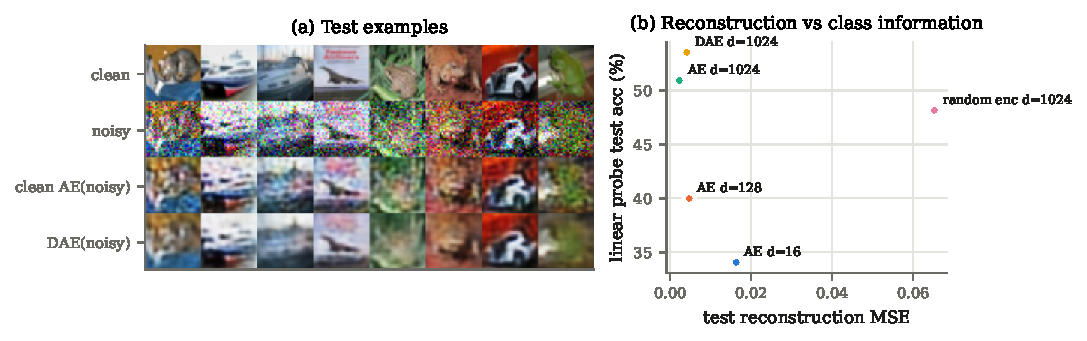
\includegraphics[width=0.85\textwidth]{q3.pdf}
\caption{Q3: test reconstructions (left), and linear-probe accuracy against reconstruction error (right).}\label{fig:q3}\end{figure*}
Decision rule: the two quantities ``agree'' if ranking the three AEs by test MSE gives the same order as ranking them
by probe accuracy, and the DAE does not reverse the relation. \ConcQthreeC

% =========================================================================== 5
\section{Q4 (bonus): SVMs and clustering}
\textbf{Representation.} Chosen before any SVM is fitted: the Q3 encoder with the highest linear-probe \emph{validation}
accuracy, \emph{\QfourRep}. Features are standardised with statistics from the subset. Because of cost, a fixed stratified
subset of \QfourSubset{} training images is drawn with the split seed before model selection and saved
(\texttt{splits/q4\_subset.npz}). It is used for every SVM; validation uses all 5k images.

\textbf{(a) $C$ and kernel.} Linear, cubic-polynomial and RBF kernels ($\gamma=$\texttt{scale}), with
$C\in\{10^{-2},\dots,10^{3}\}$ (five orders of magnitude).
\input{\gen/q4a.tex}
\begin{figure*}[t]\centering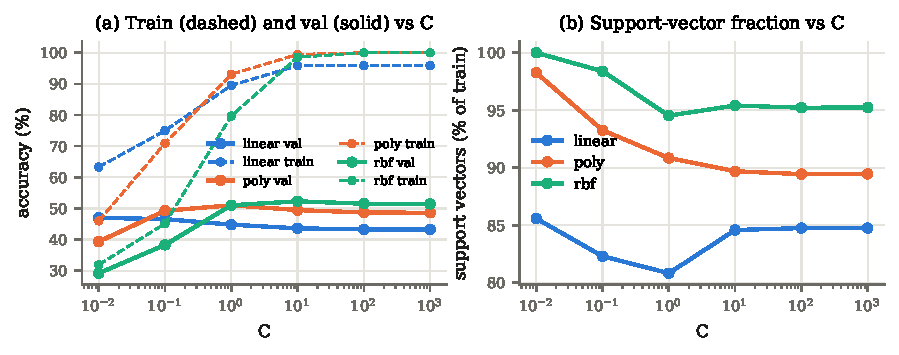
\includegraphics[width=\textwidth]{q4a.pdf}
\caption{Q4(a) validation/training accuracy and support-vector fraction against $C$ for each kernel.}\label{fig:q4a}\end{figure*}
\ConcQfourA

\textbf{(b) Difficult pairs.} The three most-confused test pairs are analysed with the pair's own one-vs-one decision
function $f_{ij}$, extracted from the fitted SVC and verified numerically against \texttt{decision\_function}.
\input{\gen/q4b.tex}
\begin{figure}[t]\centering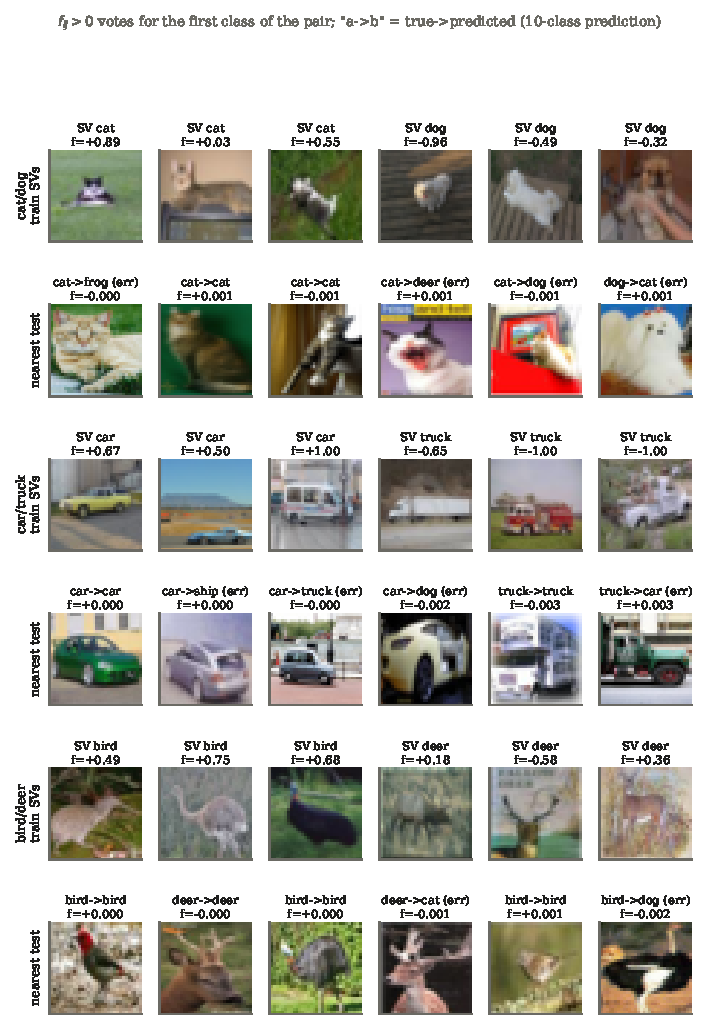
\includegraphics[width=\linewidth]{q4b_pairs.pdf}
\caption{Q4(b) training support vectors with the largest $|\alpha|$ and the test images closest to the $i$/$j$ boundary.}\label{fig:q4b}\end{figure}
\ConcQfourB

\textbf{(c) Clustering.} K-means and diagonal-covariance GMMs are fitted on training representations without labels, for
$k\in\{5,8,10,12,15,20\}$. The method and $k$ are chosen by the highest validation silhouette (label-free). The selected
model (\QfourClu) assigns the test representations; labels are used only afterwards. Test ARI is \QfourARI, NMI \QfourNMI,
purity \QfourPurity\%, and accuracy after a train-label majority mapping \QfourMapAcc\%.
\input{\gen/q4c_sel.tex}
\begin{figure}[t]\centering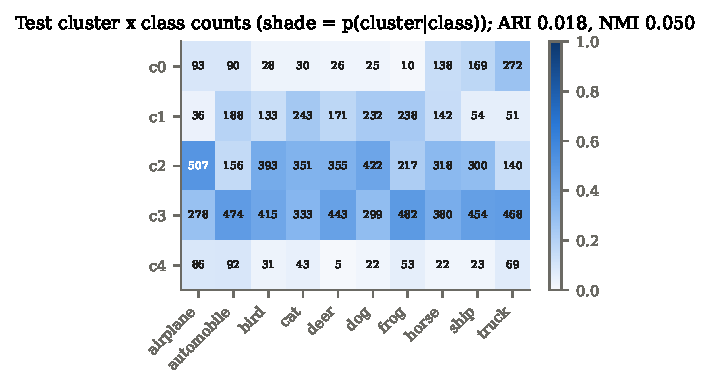
\includegraphics[width=\linewidth]{q4c_contingency.pdf}
\caption{Q4(c) test cluster-to-class contingency table.}\label{fig:q4c}\end{figure}
\input{\gen/q4c_perclass.tex}
\ConcQfourC

% =========================================================================== 6
\section{Reproducibility}
\texttt{bash scripts/run\_all.sh} reproduces every number. The environment is in \texttt{environment.yml}; split indices,
the Q4 subset, configs, per-epoch logs (\texttt{results/runs/*.json}) and figure scripts are in the repository at the
commit shown on page~1.

\end{document}
") ----
\ifdefined\smoke
  \def\gen{generated_smoke}\graphicspath{{../figures_smoke/}}
\else
  \def\gen{generated}\graphicspath{{../figures/}}
\fi
\input{\gen/numbers.tex}
\providecommand{\QtwoBlockC}{--}

% ---- conclusions are generated by the pre-registered decision rules in src/conclusions.py ----
\input{\gen/conclusions.tex}
\newcommand{\pred}[1]{\textit{Prediction (fixed before training, PREDICTIONS.md):} #1}

\title{Inductive Bias, Memorisation, Representations and Margins on CIFAR10}
\author{\StudentName\\ Roll no.\ \RollNumber\\ {\small Code: \RepoURL\quad Commit: \texttt{\CommitHash}}}
\date{}

\begin{document}
\maketitle

\begin{abstract}
We study why multilayer perceptrons (MLPs) underperform on CIFAR10 and test the explanation with equal-budget
controls, a pixel-permutation ablation and a label-noise memorisation experiment tracked across training.
We then compare a parameter-matched CNN with the MLP, probe what the CNN relies on with per-image block shuffles,
study convolutional autoencoders (bottleneck size, denoising, linear probes), and analyse SVMs and clustering on a
fixed learned representation. Every reported number is generated from the logged runs in the repository.
\end{abstract}

% =========================================================================== 1
\section{Common setup}
\textbf{Data.} The 50{,}000 CIFAR10 training images are split once into a stratified 45{,}000/5{,}000 train/validation
split with \texttt{sklearn.train\_test\_split(stratify=y)} and seed \SplitSeed{} (all digits of roll number \RollNumber,
in order). The split indices are saved in \texttt{splits/cifar10\_split.npz} and reused by every experiment.
Per-channel mean/std are computed on the 45k training images only. The validation set is the only signal for any choice
(learning rate, checkpoint epoch, bottleneck, kernel, $C$, clustering method, $k$). The official test set is evaluated
only after a choice is fixed.

\textbf{Shared training protocol.} Every classifier (all MLPs, the Patch-MLP and all CNNs) is trained by the same function
(\texttt{src/common.py:train\_classifier}): AdamW, weight decay $5\cdot10^{-4}$, batch 256, one warm-up epoch then cosine
decay, no data augmentation, and the checkpoint with the best validation accuracy. No augmentation is a deliberate choice:
random crops/flips inject a translation prior into the \emph{data}, which would confound the inductive-bias questions in
Q1/Q2. Every model receives the same tuning budget: the LR grid $\{10^{-3},3\cdot10^{-4}\}$ is searched at seed 0, and
the selected LR is re-run with seeds 1 and 2; we report mean$\pm$sd over three seeds.

\textbf{Reuse.} Models are cached by name in \texttt{results/checkpoints}. Reused components are marked where used:
the Q1(a) MLP and its pixel-permuted runs are reused in Q2; the Q2(a) seed-0 CNN is the fixed classifier in Q3(b);
the Q3 encoders provide the Q4 representation.

% =========================================================================== 2
\section{Q1: Why MLPs struggle, and memorisation}
\subsection{(a) Separating the explanations}
\textbf{Chosen reason (H\textsubscript{bias}).} A fully connected layer treats the 3072 inputs as an unordered vector.
It has no locality and no weight sharing, so a detector learned at one image position cannot be reused at another, and
neighbouring pixels are not known to be related. With 45k images the MLP can fit the training set but generalises poorly.

\textbf{Competing explanations.} H\textsubscript{cap}: the MLP lacks capacity and \emph{underfits}.
H\textsubscript{opt}: the one-hidden-layer shape is the problem and a deeper MLP of the same size would fix it.

\textbf{Design.} Three models are matched to the same parameter budget by binary-searching their width
(\cref{tab:q1spec}). The plain MLP is the baseline. The deep MLP keeps the budget and only changes depth (tests
H\textsubscript{opt}). The Patch-MLP is still built only from Linear layers. Its single change is a minimal spatial
prior: one small MLP, shared across positions, embeds every $4\times4$ patch, and a fully connected head then reads all
patch embeddings (tests H\textsubscript{bias}). Two further diagnostics are used. (i) A width sweep of the plain MLP: if
H\textsubscript{cap} held, validation accuracy would keep rising with width. Here the parameter count varies by design,
and only validation is used. (ii) A fixed pixel permutation applied to train, validation and test. If the Patch-MLP's gain
comes from spatial structure, it must vanish under permutation, while the plain MLP's accuracy is unchanged.

\textbf{Fairness.} We call the comparison fair when parameters are within 2\%, the data and preprocessing are identical,
and the epochs, optimiser, schedule, LR grid, seeds and selection rule are identical. Compute (MACs) is not matched: weight
sharing reuses parameters, and that reuse is the property under test.

\input{\gen/q1a_spec.tex}
\input{\gen/q1a.tex}
\input{\gen/q1a_capacity.tex}
\begin{figure*}[t]\centering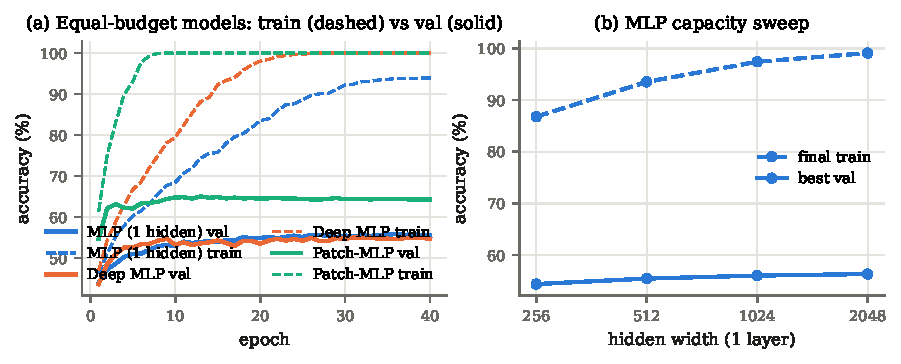
\includegraphics[width=\textwidth]{q1a_curves.pdf}
\caption{Q1(a) seed-0 training curves at the selected LR (left) and the MLP width sweep (right).}\label{fig:q1a}\end{figure*}

\textbf{Evidence.} The plain MLP reaches \QoneTrainmlp\% training accuracy at its selected epoch but only \QoneValmlp\%
validation accuracy. Its test accuracy is \QoneTestmlp\%. Deep MLP: \QoneTestmlpdeep\%; Patch-MLP: \QoneTestpatchmlp\%
(\cref{tab:q1a,tab:q1cap,fig:q1a}). Each hypothesis is judged by the rule fixed in \texttt{PREDICTIONS.md}.
\ConcQoneA

\subsection{(b) Is structure learned before memorisation?}
\textbf{Setting.} A \QoneBParams-parameter MLP (two hidden layers of width 2048) has more than enough capacity to fit 45k
examples. It is trained for 150 epochs at a constant LR with no weight decay. A fixed 40\% of the training labels (seeded)
are replaced by a uniformly random \emph{wrong} class; these examples cannot generalise by construction. At every epoch we
measure, on the training set: accuracy on the clean subset; agreement of the noisy subset with its noisy label
(memorisation); agreement of the noisy subset with its hidden true label (structure); and clean validation accuracy. A
clean-label run with an identical protocol is the control. We also record, for every example, the epoch from which it
stays fitted until the end of training (\cref{fig:q1b}b).

\input{\gen/q1b.tex}
\begin{figure*}[t]\centering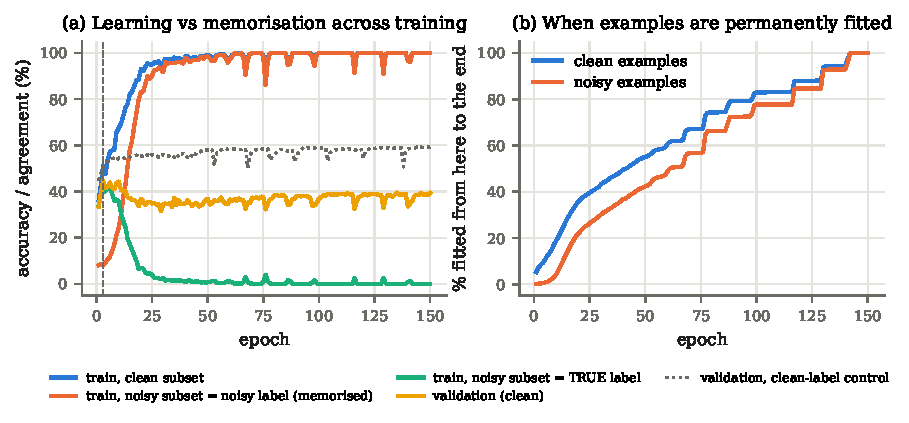
\includegraphics[width=\textwidth]{q1b_memorisation.pdf}
\caption{Q1(b) per-epoch measurements under 40\% label noise. The dashed vertical line marks peak validation accuracy.}\label{fig:q1b}\end{figure*}

\textbf{Evidence.} Validation accuracy peaks at epoch \QoneBPeakEpoch{} (\QoneBPeakVal\%). At that epoch only
\QoneBPeakNoisyFit\% of the corrupted examples are predicted as their noisy label, while \QoneBPeakNoisyTrue\% are
predicted as their \emph{true} class. The noisy-fit fraction first exceeds 50\% at epoch \QoneBOnsetFifty. \ConcQoneB{} \Cref{fig:q1b}b shows the same
ordering per example: the epoch from which an example stays fitted is early for clean examples and late for corrupted
ones. The test accuracy of the val-selected checkpoint
is \QoneBTest\%.

% =========================================================================== 3
\section{Q2: CNN vs MLP}
\textbf{Fairness criterion (fixed before training).} The CNN's width is binary-searched so that its parameter count
matches the Q1 MLP (\QtwoCNNparams{} vs \QtwoMLPparams). Everything else follows the shared protocol of Q1. The Q1(a)
plain MLP and its runs are \emph{reused} unchanged as the Q2 MLP. The CNN uses about \QtwoMACratio$\times$ more MACs per
image; we report this rather than hide it.

\input{\gen/q2.tex}

\textbf{(a) Result and proposed reason.} The CNN reaches \QtwoCNNclean\% test accuracy and the MLP \QtwoMLPclean\%.
The proposed reason is the same spatial prior identified in Q1: local receptive fields with shared weights reuse one
feature detector at every position, so far fewer examples are needed per feature.

\textbf{(b) Spatial disturbance.} We apply one fixed permutation of the 1024 pixel positions, identical for every
training, validation and test image. RGB triplets move together, so all pixel values and colours are preserved exactly.
\pred{the MLP is unchanged within seed noise, because a fixed input permutation can be absorbed into its first layer; the
CNN falls to roughly the MLP level or below.} Observed: MLP \QtwoMLPperm\%, CNN \QtwoCNNperm\%. \ConcQtwoB

\textbf{(c) Which spatial information does the CNN use?}
E\textsubscript{local}: the CNN classifies from local texture and colour statistics, like a bag of local features.
E\textsubscript{global}: it needs the global arrangement of object parts. We cut every image into $b\times b$ tiles
($b\in\{16,8,4\}$) and shuffle the tiles with a permutation that differs per image (deterministic from a seed). This keeps
the content inside each tile and destroys the global layout. The CNN is retrained per condition. The identical
transformation (same operator, block size and seeded generator) is applied to training, validation and test images; as with
any random transformation, only the per-image draw differs. \pred{under E\textsubscript{local}, accuracy and confidence largely
survive at $b=16$ and $b=8$ and fall at $b=4$, when tiles become smaller than parts. Under E\textsubscript{global}, there is
already a large drop at $b=16$.}

\input{\gen/q2_conf.tex}
\begin{figure*}[t]\centering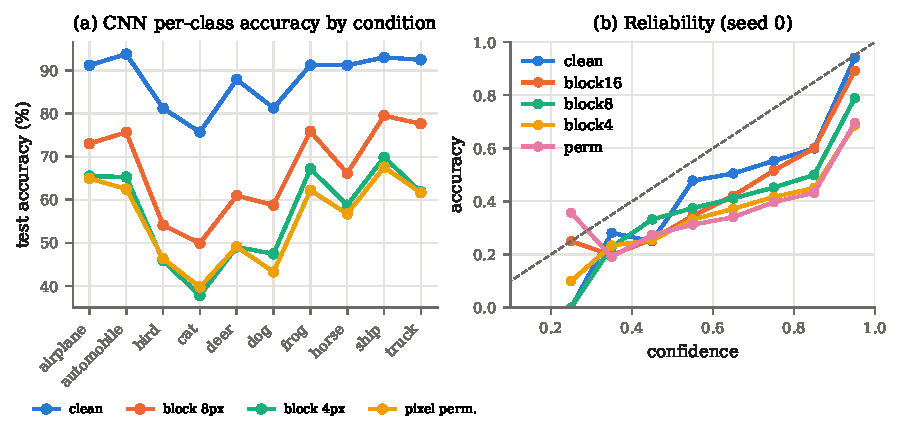
\includegraphics[width=\textwidth]{q2_analysis.pdf}
\caption{Q2(c): per-class test accuracy and reliability diagrams for the CNN across conditions.}\label{fig:q2}\end{figure*}

Decision rule (pre-registered): E\textsubscript{local} if the drop at 16\,px is $<$40\% of the drop at 4\,px,
E\textsubscript{global} if $\ge$60\%, otherwise both. \ConcQtwoC

\textbf{Conclusion linking the three experiments.} \ConcQtwoLink

% =========================================================================== 4
\section{Q3: Autoencoders}
\textbf{(a) Bottleneck capacity.} The three ConvAEs share one encoder (three stride-2 conv layers, $32\to4$ px, 2048
values), a Linear bottleneck of size $d\in\{16,128,1024\}$ and a mirrored decoder with a sigmoid output. Only $d$ changes.
Training uses MSE on $[0,1]$ pixels, AdamW at LR $10^{-3}$, cosine decay and 40 epochs; the checkpoint is the epoch with
the lowest validation MSE. Selection rule: lowest validation MSE. The selected model is $d=\QthreeSel$, with test MSE
\QthreeTestMSE{} (PSNR \QthreeTestPSNR{} dB).
\input{\gen/q3a.tex}

\textbf{(b) Denoising.} Corruption: additive Gaussian noise, $\sigma=0.2$, clipped to $[0,1]$. Reconstruction can
plausibly help because the noise is independent per pixel while natural images are spatially smooth. Protocol: the DAE has
the same architecture as the selected AE. Its input is a freshly noised training image in every batch, the target is the
clean image, and no labels are used. Validation and test noise are drawn once with fixed seeds. The fixed classifier is the
Q2(a) seed-0 CNN (\emph{reused}, never fine-tuned).
\input{\gen/q3b.tex}
Decision rule (pre-registered): the DAE ``recovers the information the classifier needs'' if it closes $\ge$50\% of
the clean--noisy gap \emph{and} comes within 3\,pp of the ``clean AE on clean'' ceiling. \ConcQthreeB

\textbf{(c) Class information vs reconstruction.} The encoders are frozen. Bottleneck features of the three AEs, the DAE
and a randomly initialised encoder (control) are classified with an L2-regularised linear softmax probe (strength chosen
on validation) and with 20-NN.
\input{\gen/q3c.tex}
\begin{figure*}[t]\centering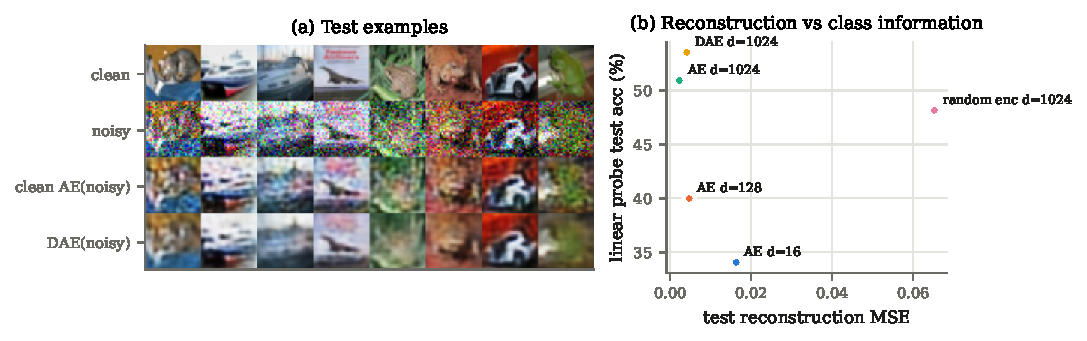
\includegraphics[width=0.85\textwidth]{q3.pdf}
\caption{Q3: test reconstructions (left), and linear-probe accuracy against reconstruction error (right).}\label{fig:q3}\end{figure*}
Decision rule: the two quantities ``agree'' if ranking the three AEs by test MSE gives the same order as ranking them
by probe accuracy, and the DAE does not reverse the relation. \ConcQthreeC

% =========================================================================== 5
\section{Q4 (bonus): SVMs and clustering}
\textbf{Representation.} Chosen before any SVM is fitted: the Q3 encoder with the highest linear-probe \emph{validation}
accuracy, \emph{\QfourRep}. Features are standardised with statistics from the subset. Because of cost, a fixed stratified
subset of \QfourSubset{} training images is drawn with the split seed before model selection and saved
(\texttt{splits/q4\_subset.npz}). It is used for every SVM; validation uses all 5k images.

\textbf{(a) $C$ and kernel.} Linear, cubic-polynomial and RBF kernels ($\gamma=$\texttt{scale}), with
$C\in\{10^{-2},\dots,10^{3}\}$ (five orders of magnitude).
\input{\gen/q4a.tex}
\begin{figure*}[t]\centering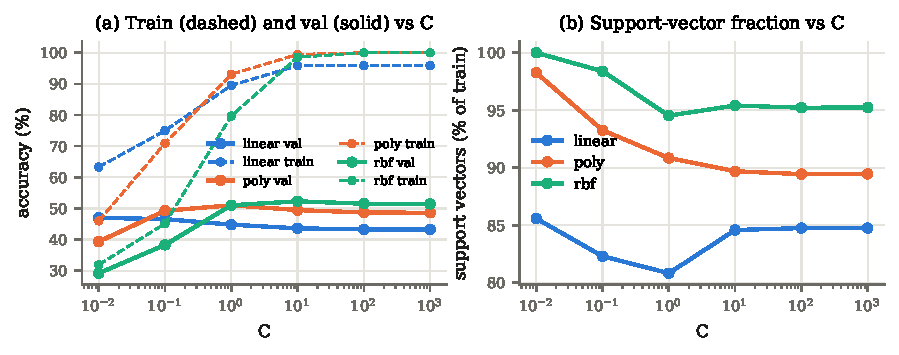
\includegraphics[width=\textwidth]{q4a.pdf}
\caption{Q4(a) validation/training accuracy and support-vector fraction against $C$ for each kernel.}\label{fig:q4a}\end{figure*}
\ConcQfourA

\textbf{(b) Difficult pairs.} The three most-confused test pairs are analysed with the pair's own one-vs-one decision
function $f_{ij}$, extracted from the fitted SVC and verified numerically against \texttt{decision\_function}.
\input{\gen/q4b.tex}
\begin{figure}[t]\centering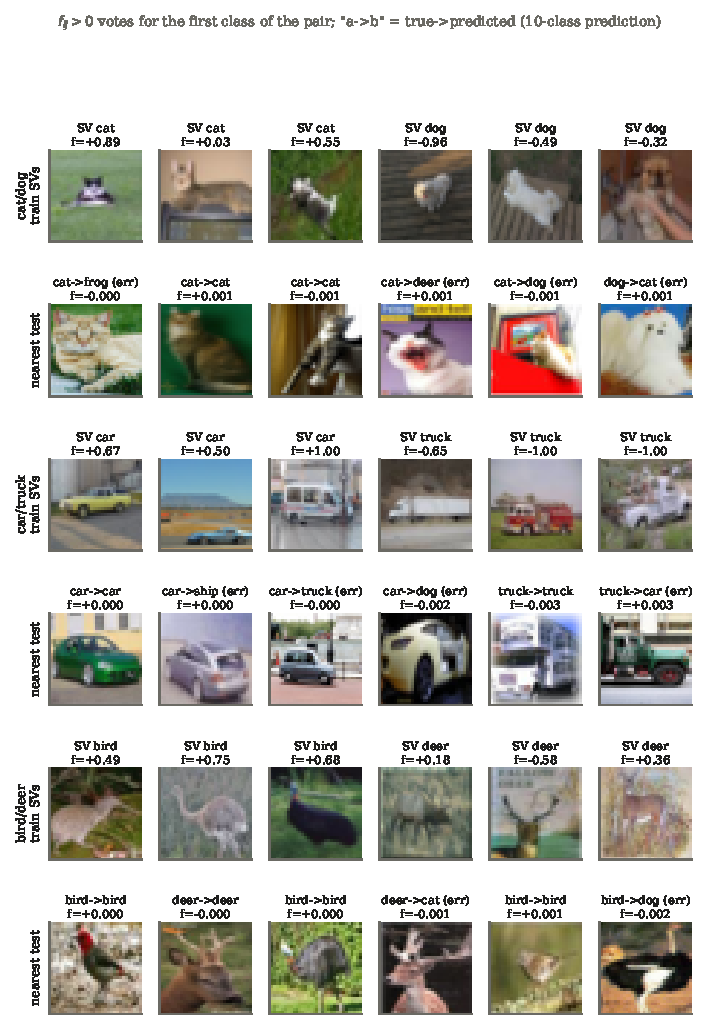
\includegraphics[width=\linewidth]{q4b_pairs.pdf}
\caption{Q4(b) training support vectors with the largest $|\alpha|$ and the test images closest to the $i$/$j$ boundary.}\label{fig:q4b}\end{figure}
\ConcQfourB

\textbf{(c) Clustering.} K-means and diagonal-covariance GMMs are fitted on training representations without labels, for
$k\in\{5,8,10,12,15,20\}$. The method and $k$ are chosen by the highest validation silhouette (label-free). The selected
model (\QfourClu) assigns the test representations; labels are used only afterwards. Test ARI is \QfourARI, NMI \QfourNMI,
purity \QfourPurity\%, and accuracy after a train-label majority mapping \QfourMapAcc\%.
\input{\gen/q4c_sel.tex}
\begin{figure}[t]\centering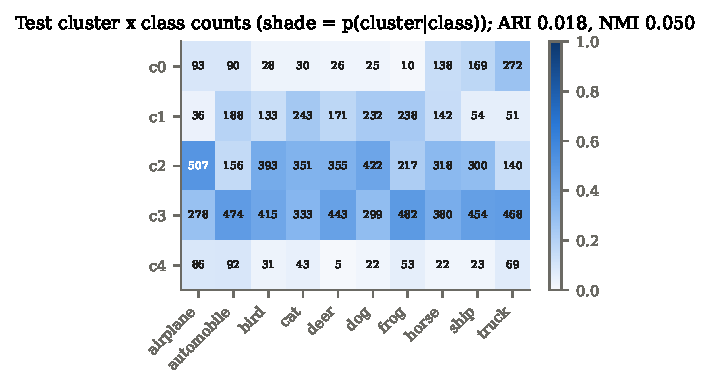
\includegraphics[width=\linewidth]{q4c_contingency.pdf}
\caption{Q4(c) test cluster-to-class contingency table.}\label{fig:q4c}\end{figure}
\input{\gen/q4c_perclass.tex}
\ConcQfourC

% =========================================================================== 6
\section{Reproducibility}
\texttt{bash scripts/run\_all.sh} reproduces every number. The environment is in \texttt{environment.yml}; split indices,
the Q4 subset, configs, per-epoch logs (\texttt{results/runs/*.json}) and figure scripts are in the repository at the
commit shown on page~1.

\end{document}
") ----
\ifdefined\smoke
  \def\gen{generated_smoke}\graphicspath{{../figures_smoke/}}
\else
  \def\gen{generated}\graphicspath{{../figures/}}
\fi
\input{\gen/numbers.tex}
\providecommand{\QtwoBlockC}{--}

% ---- conclusions are generated by the pre-registered decision rules in src/conclusions.py ----
\input{\gen/conclusions.tex}
\newcommand{\pred}[1]{\textit{Prediction (fixed before training, PREDICTIONS.md):} #1}

\title{Inductive Bias, Memorisation, Representations and Margins on CIFAR10}
\author{\StudentName\\ Roll no.\ \RollNumber\\ {\small Code: \RepoURL\quad Commit: \texttt{\CommitHash}}}
\date{}

\begin{document}
\maketitle

\begin{abstract}
We study why multilayer perceptrons (MLPs) underperform on CIFAR10 and test the explanation with equal-budget
controls, a pixel-permutation ablation and a label-noise memorisation experiment tracked across training.
We then compare a parameter-matched CNN with the MLP, probe what the CNN relies on with per-image block shuffles,
study convolutional autoencoders (bottleneck size, denoising, linear probes), and analyse SVMs and clustering on a
fixed learned representation. Every reported number is generated from the logged runs in the repository.
\end{abstract}

% =========================================================================== 1
\section{Common setup}
\textbf{Data.} The 50{,}000 CIFAR10 training images are split once into a stratified 45{,}000/5{,}000 train/validation
split with \texttt{sklearn.train\_test\_split(stratify=y)} and seed \SplitSeed{} (all digits of roll number \RollNumber,
in order). The split indices are saved in \texttt{splits/cifar10\_split.npz} and reused by every experiment.
Per-channel mean/std are computed on the 45k training images only. The validation set is the only signal for any choice
(learning rate, checkpoint epoch, bottleneck, kernel, $C$, clustering method, $k$). The official test set is evaluated
only after a choice is fixed.

\textbf{Shared training protocol.} Every classifier (all MLPs, the Patch-MLP and all CNNs) is trained by the same function
(\texttt{src/common.py:train\_classifier}): AdamW, weight decay $5\cdot10^{-4}$, batch 256, one warm-up epoch then cosine
decay, no data augmentation, and the checkpoint with the best validation accuracy. No augmentation is a deliberate choice:
random crops/flips inject a translation prior into the \emph{data}, which would confound the inductive-bias questions in
Q1/Q2. Every model receives the same tuning budget: the LR grid $\{10^{-3},3\cdot10^{-4}\}$ is searched at seed 0, and
the selected LR is re-run with seeds 1 and 2; we report mean$\pm$sd over three seeds.

\textbf{Reuse.} Models are cached by name in \texttt{results/checkpoints}. Reused components are marked where used:
the Q1(a) MLP and its pixel-permuted runs are reused in Q2; the Q2(a) seed-0 CNN is the fixed classifier in Q3(b);
the Q3 encoders provide the Q4 representation.

% =========================================================================== 2
\section{Q1: Why MLPs struggle, and memorisation}
\subsection{(a) Separating the explanations}
\textbf{Chosen reason (H\textsubscript{bias}).} A fully connected layer treats the 3072 inputs as an unordered vector.
It has no locality and no weight sharing, so a detector learned at one image position cannot be reused at another, and
neighbouring pixels are not known to be related. With 45k images the MLP can fit the training set but generalises poorly.

\textbf{Competing explanations.} H\textsubscript{cap}: the MLP lacks capacity and \emph{underfits}.
H\textsubscript{opt}: the one-hidden-layer shape is the problem and a deeper MLP of the same size would fix it.

\textbf{Design.} Three models are matched to the same parameter budget by binary-searching their width
(\cref{tab:q1spec}). The plain MLP is the baseline. The deep MLP keeps the budget and only changes depth (tests
H\textsubscript{opt}). The Patch-MLP is still built only from Linear layers. Its single change is a minimal spatial
prior: one small MLP, shared across positions, embeds every $4\times4$ patch, and a fully connected head then reads all
patch embeddings (tests H\textsubscript{bias}). Two further diagnostics are used. (i) A width sweep of the plain MLP: if
H\textsubscript{cap} held, validation accuracy would keep rising with width. Here the parameter count varies by design,
and only validation is used. (ii) A fixed pixel permutation applied to train, validation and test. If the Patch-MLP's gain
comes from spatial structure, it must vanish under permutation, while the plain MLP's accuracy is unchanged.

\textbf{Fairness.} We call the comparison fair when parameters are within 2\%, the data and preprocessing are identical,
and the epochs, optimiser, schedule, LR grid, seeds and selection rule are identical. Compute (MACs) is not matched: weight
sharing reuses parameters, and that reuse is the property under test.

\input{\gen/q1a_spec.tex}
\input{\gen/q1a.tex}
\input{\gen/q1a_capacity.tex}
\begin{figure*}[t]\centering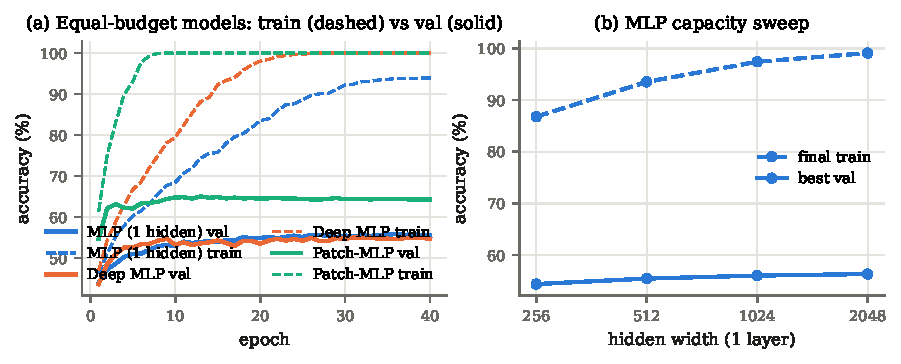
\includegraphics[width=\textwidth]{q1a_curves.pdf}
\caption{Q1(a) seed-0 training curves at the selected LR (left) and the MLP width sweep (right).}\label{fig:q1a}\end{figure*}

\textbf{Evidence.} The plain MLP reaches \QoneTrainmlp\% training accuracy at its selected epoch but only \QoneValmlp\%
validation accuracy. Its test accuracy is \QoneTestmlp\%. Deep MLP: \QoneTestmlpdeep\%; Patch-MLP: \QoneTestpatchmlp\%
(\cref{tab:q1a,tab:q1cap,fig:q1a}). Each hypothesis is judged by the rule fixed in \texttt{PREDICTIONS.md}.
\ConcQoneA

\subsection{(b) Is structure learned before memorisation?}
\textbf{Setting.} A \QoneBParams-parameter MLP (two hidden layers of width 2048) has more than enough capacity to fit 45k
examples. It is trained for 150 epochs at a constant LR with no weight decay. A fixed 40\% of the training labels (seeded)
are replaced by a uniformly random \emph{wrong} class; these examples cannot generalise by construction. At every epoch we
measure, on the training set: accuracy on the clean subset; agreement of the noisy subset with its noisy label
(memorisation); agreement of the noisy subset with its hidden true label (structure); and clean validation accuracy. A
clean-label run with an identical protocol is the control. We also record, for every example, the epoch from which it
stays fitted until the end of training (\cref{fig:q1b}b).

\input{\gen/q1b.tex}
\begin{figure*}[t]\centering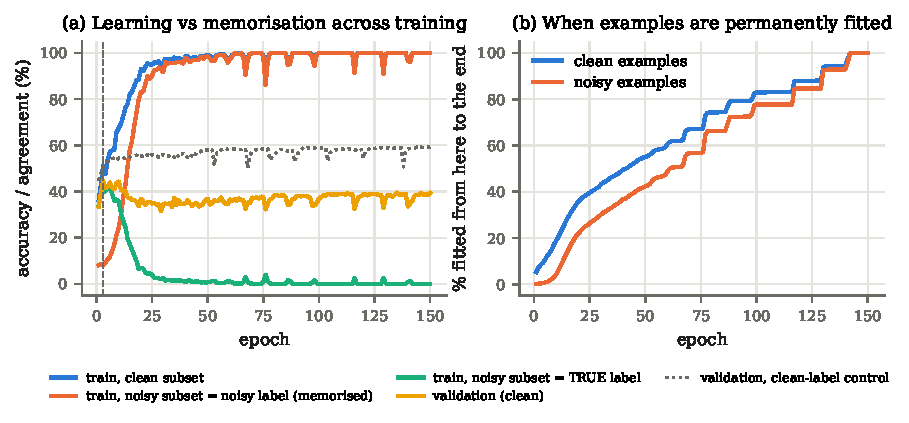
\includegraphics[width=\textwidth]{q1b_memorisation.pdf}
\caption{Q1(b) per-epoch measurements under 40\% label noise. The dashed vertical line marks peak validation accuracy.}\label{fig:q1b}\end{figure*}

\textbf{Evidence.} Validation accuracy peaks at epoch \QoneBPeakEpoch{} (\QoneBPeakVal\%). At that epoch only
\QoneBPeakNoisyFit\% of the corrupted examples are predicted as their noisy label, while \QoneBPeakNoisyTrue\% are
predicted as their \emph{true} class. The noisy-fit fraction first exceeds 50\% at epoch \QoneBOnsetFifty. \ConcQoneB{} \Cref{fig:q1b}b shows the same
ordering per example: the epoch from which an example stays fitted is early for clean examples and late for corrupted
ones. The test accuracy of the val-selected checkpoint
is \QoneBTest\%.

% =========================================================================== 3
\section{Q2: CNN vs MLP}
\textbf{Fairness criterion (fixed before training).} The CNN's width is binary-searched so that its parameter count
matches the Q1 MLP (\QtwoCNNparams{} vs \QtwoMLPparams). Everything else follows the shared protocol of Q1. The Q1(a)
plain MLP and its runs are \emph{reused} unchanged as the Q2 MLP. The CNN uses about \QtwoMACratio$\times$ more MACs per
image; we report this rather than hide it.

\input{\gen/q2.tex}

\textbf{(a) Result and proposed reason.} The CNN reaches \QtwoCNNclean\% test accuracy and the MLP \QtwoMLPclean\%.
The proposed reason is the same spatial prior identified in Q1: local receptive fields with shared weights reuse one
feature detector at every position, so far fewer examples are needed per feature.

\textbf{(b) Spatial disturbance.} We apply one fixed permutation of the 1024 pixel positions, identical for every
training, validation and test image. RGB triplets move together, so all pixel values and colours are preserved exactly.
\pred{the MLP is unchanged within seed noise, because a fixed input permutation can be absorbed into its first layer; the
CNN falls to roughly the MLP level or below.} Observed: MLP \QtwoMLPperm\%, CNN \QtwoCNNperm\%. \ConcQtwoB

\textbf{(c) Which spatial information does the CNN use?}
E\textsubscript{local}: the CNN classifies from local texture and colour statistics, like a bag of local features.
E\textsubscript{global}: it needs the global arrangement of object parts. We cut every image into $b\times b$ tiles
($b\in\{16,8,4\}$) and shuffle the tiles with a permutation that differs per image (deterministic from a seed). This keeps
the content inside each tile and destroys the global layout. The CNN is retrained per condition. The identical
transformation (same operator, block size and seeded generator) is applied to training, validation and test images; as with
any random transformation, only the per-image draw differs. \pred{under E\textsubscript{local}, accuracy and confidence largely
survive at $b=16$ and $b=8$ and fall at $b=4$, when tiles become smaller than parts. Under E\textsubscript{global}, there is
already a large drop at $b=16$.}

\input{\gen/q2_conf.tex}
\begin{figure*}[t]\centering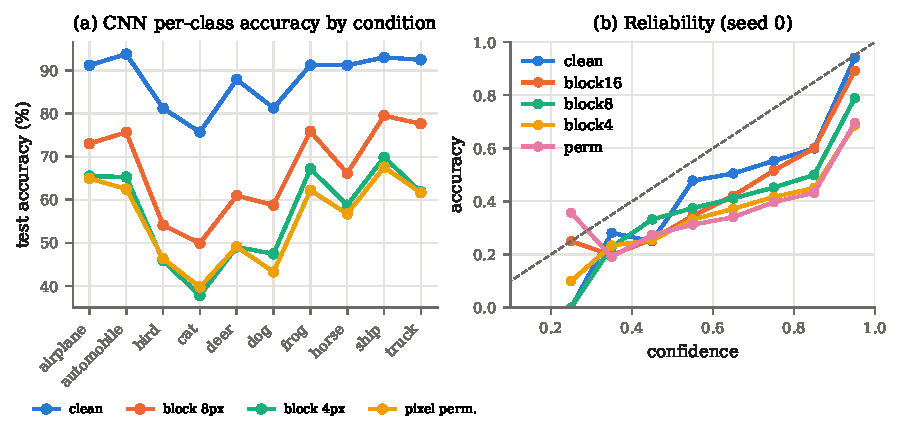
\includegraphics[width=\textwidth]{q2_analysis.pdf}
\caption{Q2(c): per-class test accuracy and reliability diagrams for the CNN across conditions.}\label{fig:q2}\end{figure*}

Decision rule (pre-registered): E\textsubscript{local} if the drop at 16\,px is $<$40\% of the drop at 4\,px,
E\textsubscript{global} if $\ge$60\%, otherwise both. \ConcQtwoC

\textbf{Conclusion linking the three experiments.} \ConcQtwoLink

% =========================================================================== 4
\section{Q3: Autoencoders}
\textbf{(a) Bottleneck capacity.} The three ConvAEs share one encoder (three stride-2 conv layers, $32\to4$ px, 2048
values), a Linear bottleneck of size $d\in\{16,128,1024\}$ and a mirrored decoder with a sigmoid output. Only $d$ changes.
Training uses MSE on $[0,1]$ pixels, AdamW at LR $10^{-3}$, cosine decay and 40 epochs; the checkpoint is the epoch with
the lowest validation MSE. Selection rule: lowest validation MSE. The selected model is $d=\QthreeSel$, with test MSE
\QthreeTestMSE{} (PSNR \QthreeTestPSNR{} dB).
\input{\gen/q3a.tex}

\textbf{(b) Denoising.} Corruption: additive Gaussian noise, $\sigma=0.2$, clipped to $[0,1]$. Reconstruction can
plausibly help because the noise is independent per pixel while natural images are spatially smooth. Protocol: the DAE has
the same architecture as the selected AE. Its input is a freshly noised training image in every batch, the target is the
clean image, and no labels are used. Validation and test noise are drawn once with fixed seeds. The fixed classifier is the
Q2(a) seed-0 CNN (\emph{reused}, never fine-tuned).
\input{\gen/q3b.tex}
Decision rule (pre-registered): the DAE ``recovers the information the classifier needs'' if it closes $\ge$50\% of
the clean--noisy gap \emph{and} comes within 3\,pp of the ``clean AE on clean'' ceiling. \ConcQthreeB

\textbf{(c) Class information vs reconstruction.} The encoders are frozen. Bottleneck features of the three AEs, the DAE
and a randomly initialised encoder (control) are classified with an L2-regularised linear softmax probe (strength chosen
on validation) and with 20-NN.
\input{\gen/q3c.tex}
\begin{figure*}[t]\centering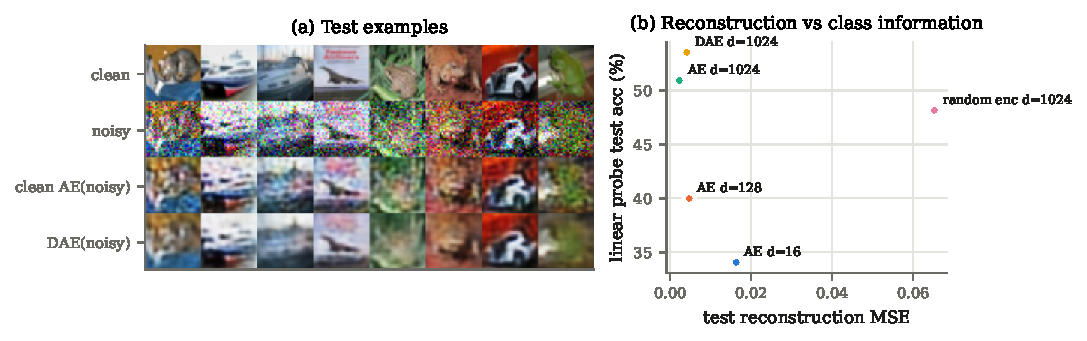
\includegraphics[width=0.85\textwidth]{q3.pdf}
\caption{Q3: test reconstructions (left), and linear-probe accuracy against reconstruction error (right).}\label{fig:q3}\end{figure*}
Decision rule: the two quantities ``agree'' if ranking the three AEs by test MSE gives the same order as ranking them
by probe accuracy, and the DAE does not reverse the relation. \ConcQthreeC

% =========================================================================== 5
\section{Q4 (bonus): SVMs and clustering}
\textbf{Representation.} Chosen before any SVM is fitted: the Q3 encoder with the highest linear-probe \emph{validation}
accuracy, \emph{\QfourRep}. Features are standardised with statistics from the subset. Because of cost, a fixed stratified
subset of \QfourSubset{} training images is drawn with the split seed before model selection and saved
(\texttt{splits/q4\_subset.npz}). It is used for every SVM; validation uses all 5k images.

\textbf{(a) $C$ and kernel.} Linear, cubic-polynomial and RBF kernels ($\gamma=$\texttt{scale}), with
$C\in\{10^{-2},\dots,10^{3}\}$ (five orders of magnitude).
\input{\gen/q4a.tex}
\begin{figure*}[t]\centering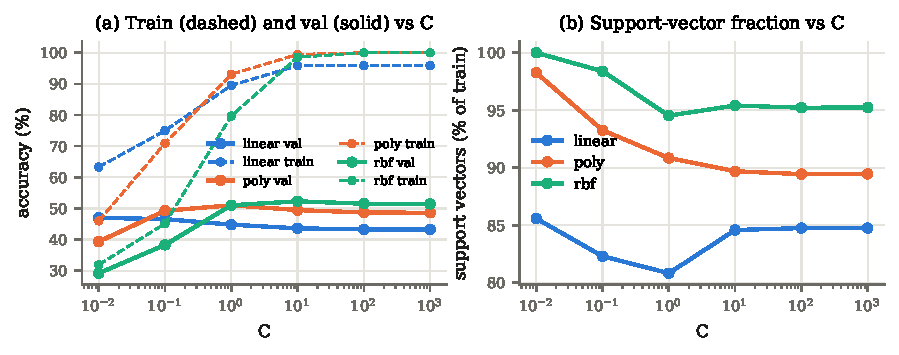
\includegraphics[width=\textwidth]{q4a.pdf}
\caption{Q4(a) validation/training accuracy and support-vector fraction against $C$ for each kernel.}\label{fig:q4a}\end{figure*}
\ConcQfourA

\textbf{(b) Difficult pairs.} The three most-confused test pairs are analysed with the pair's own one-vs-one decision
function $f_{ij}$, extracted from the fitted SVC and verified numerically against \texttt{decision\_function}.
\input{\gen/q4b.tex}
\begin{figure}[t]\centering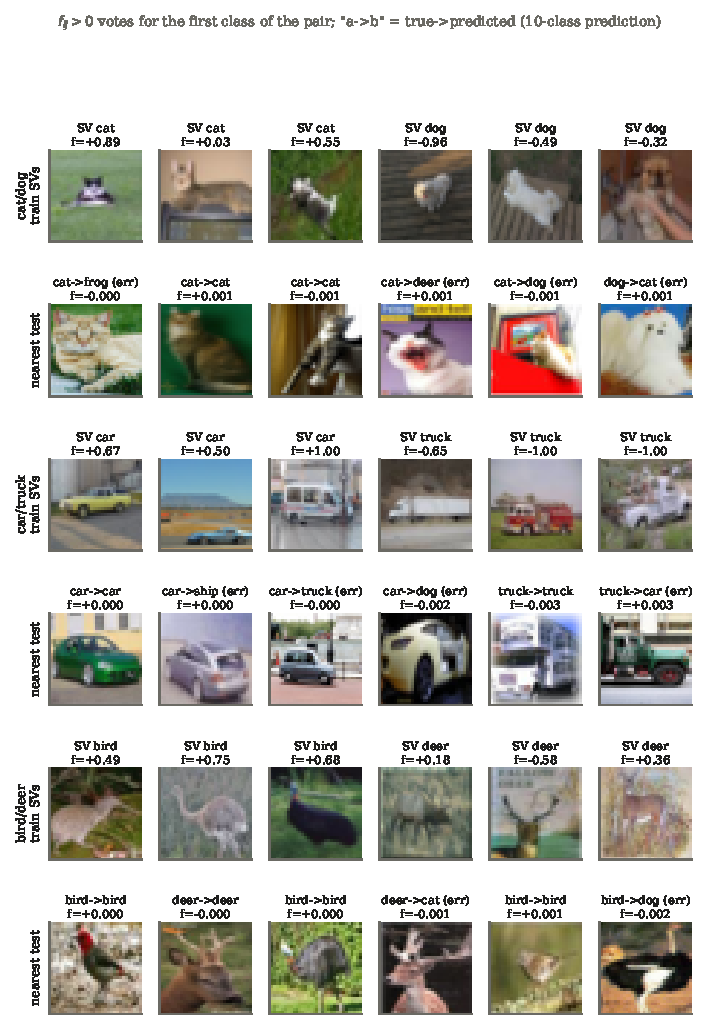
\includegraphics[width=\linewidth]{q4b_pairs.pdf}
\caption{Q4(b) training support vectors with the largest $|\alpha|$ and the test images closest to the $i$/$j$ boundary.}\label{fig:q4b}\end{figure}
\ConcQfourB

\textbf{(c) Clustering.} K-means and diagonal-covariance GMMs are fitted on training representations without labels, for
$k\in\{5,8,10,12,15,20\}$. The method and $k$ are chosen by the highest validation silhouette (label-free). The selected
model (\QfourClu) assigns the test representations; labels are used only afterwards. Test ARI is \QfourARI, NMI \QfourNMI,
purity \QfourPurity\%, and accuracy after a train-label majority mapping \QfourMapAcc\%.
\input{\gen/q4c_sel.tex}
\begin{figure}[t]\centering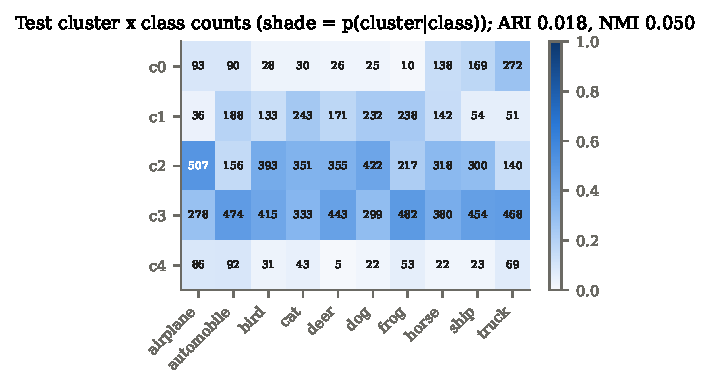
\includegraphics[width=\linewidth]{q4c_contingency.pdf}
\caption{Q4(c) test cluster-to-class contingency table.}\label{fig:q4c}\end{figure}
\input{\gen/q4c_perclass.tex}
\ConcQfourC

% =========================================================================== 6
\section{Reproducibility}
\texttt{bash scripts/run\_all.sh} reproduces every number. The environment is in \texttt{environment.yml}; split indices,
the Q4 subset, configs, per-epoch logs (\texttt{results/runs/*.json}) and figure scripts are in the repository at the
commit shown on page~1.

\end{document}
